\subsubsection{UCA 4 - Inserimento modalità di tracciamento}%kite level

\begin{figure}[h!]
	\centering	
	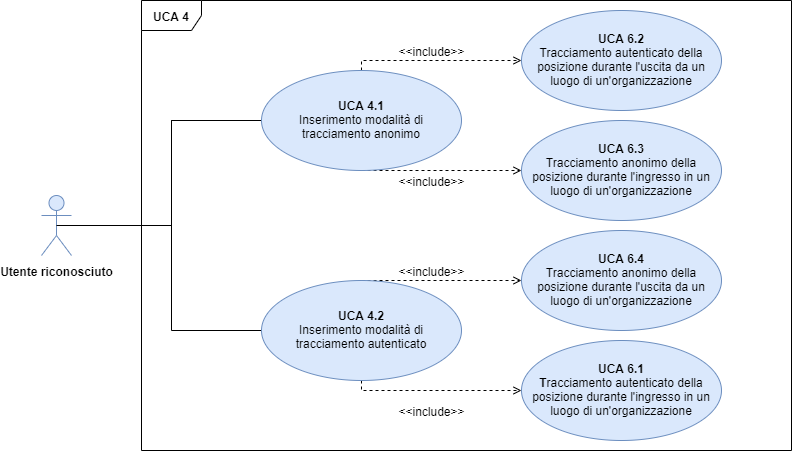
\includegraphics[scale=0.53, center]{Sezioni/UseCase/Immagini/UCA4.png}
	\caption{UCA 4 - Inserimento modalità di tracciamento}
\end{figure}

\begin{itemize}
	\item \textbf{Attori primari:} Utente riconosciuto, Utente anonimo
	\item \textbf{Precondizione:} L'utente si è autenticato con le credenziali \glo{LDAP} nella \glo{organizzazione} in cui si trova e vuole selezionare la modalità di \glo{tracciamento}.
	\item \textbf{Postcondizione:} L'utente viene tracciato secondo la modalità da lui scelta precedentemente.
	\item \textbf{Scenario principale:} L'utente vuole cambiare modalità di \glo{tracciamento} accedendone alla funzionalità.
	\item \textbf{Flusso di eventi:}
	\begin{enumerate}
		\item L'utente accede alla funzione di inserimento modalità di \glo{tracciamento};
		\item L'utente può scegliere la modalità di \glo{tracciamento anonimo} [UCA 4.1] oppure la modalità di \glo{tracciamento autenticato} [UCA 4.2].
	\end{enumerate}
\end{itemize}

\subsubsection{UCA 4.1 - Inserimento modalità di tracciamento anonimo}%sea level
\begin{itemize}
	\item \textbf{Attori primari:} Utente riconosciuto
	\item \textbf{Precondizione:} L'utente riconosciuto ha effettuato l'accesso alla funzione di inserimento modalità di \glo{tracciamento}.
	\item \textbf{Postcondizione:} L'utente viene tracciato secondo la \glo{modalità di tracciamento anonimo}.
	\item \textbf{Scenario principale:} L'utente inserisce la \glo{modalità di tracciamento anonimo}.
\end{itemize}

\subsubsection{UCA 4.2 - Inserimento modalità di tracciamento autenticato}%sea level
\begin{itemize}
	\item \textbf{Attori primari:} Utente anonimo
	\item \textbf{Precondizione:} L'utente anonimo ha effettuato l'accesso alla funzione di inserimento modalità di \glo{tracciamento}.
	\item \textbf{Postcondizione:} L'utente viene tracciato secondo la \glo{modalità di tracciamento anonimo}.
	\item \textbf{Scenario principale:} L'utente inserisce la \glo{modalità di tracciamento autenticato}.
\end{itemize}
